\begin{center}
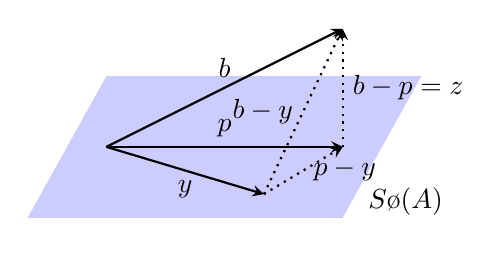
\begin{tikzpicture}
	\tikzset{>=stealth}
	\fill[blue!20] (0,0) -- (1,1.8) -- (5,1.8) -- (4,0) -- cycle;

	\node (sa) at (4.8,0.2) {$S\text{ø}(A)$};

	\coordinate (s) at (1,0.9);
	\coordinate (pE) at (4,0.9);
	\coordinate (bE) at (4,2.4);
	\coordinate (yE) at (3,0.3);
	
	\draw[thick,->] (s) to node[above]{$p$} (pE);
	\draw[thick,->] (s) to node[above]{$b$} (bE);
	\draw[thick,->,dotted] (pE) to node[right]{$b-p = z$} (bE);
	\draw[thick,->] (s) to node[below]{$y$} (yE);
	\draw[thick,->,dotted] (yE) to node[left]{$b-y$} (bE);
	\draw[thick,->,dotted] (yE) to node[right]{$p-y$} (pE);
\end{tikzpicture}
\end{center}
